\documentclass[13pt, a4paper, titlepage]{article}

\usepackage{polski}
\usepackage[utf8]{inputenc}
\usepackage[pdftex]{graphicx}
\usepackage{url}
\usepackage{hyperref}
\hypersetup{
colorlinks,
citecolor=[rgb]{0, 0.0, 0.0},
linkcolor=[rgb]{0,0,0},
urlcolor=blue}

\author{Rafał ~Kostun}
\title{Projekt \LaTeX}
\date{\today}
\linespread{1.2}






                    \begin{document}

\maketitle

\tableofcontents
-----------------------------------------------------------------------------------------------
\\\\\\\\\\\\\\\\\\\\\\\\\\\\\\\\\\\\\\\\\\\\\\\\\\\\
\begin{figure}[h]
\centering

\includegraphics[width=2cm]{images.jpg}
\caption{Ja podczas pisania tego dokumentu}
\label{fig:images}
\end{figure}
\newpage
\section{Wstęp}

W tym projekcie chciałbym przedstawić algorytm Gaussa-Jordana oraz podać przykład rozwiązywania układu równań tą metodą.
\\\\\\\\



        \section{Algorytm Gaussa-Jordana}
W celu rozwiązania układu równań liniowych \textbf{$Ax = b$} wykonujemy następujące kroki:

            \begin{enumerate}

  \item Tworzymy macierz rozszerzoną \textbf{$[A|b]$} układu \textbf{$Ax = b$}
  \item Macierz \textbf{$[A|b]$} redukujemy do wierszowo równoważnej macierzy chodkowej \textbf{$[C|d]$}.Jeśli \textbf{$d$} jest wiodoącą kolumną macierzy \textbf{[$[C|d]$}, układ \textbf{$Ax = b$} jest sprzeczny. W przeciwnym wypadku przechodzimy do nastepnego kroku.
  \item Wypisujemy układ rownań liniowych \textbf{$Cx = d$}.
  \item Z ukladu \textbf{$Cx = d$} metodą cofania (wprost, gdy \textbf{$[C|d]$} jest normalna macierzą schodkową) wyznaczamy niewiadome odpowiadające wiodącym kolumnom macierzy \textbf{$[C|d].$}

            \end{enumerate}
\newpage
\section{Przykład}(Fragment pochodzi z książki ,,Algebra liniowa~\cite{topp}")
\\\\
        Rozwiązemy teraz taki układ równań:

    \begin{equation}
	\left\{	
	\begin{array}{ll}

\ \ \ \ \ \ \ \ \ \ \   2x_2 - \ 8x_3  &=\ \ 8, \\

\ \ \  \ x_1 -  2x_2 +  \ \ \ x_3  &=\ \ 0, \\
-4x_1 +  5x_2 + 10x_3  &= -6, \\
		
	\end{array} \right.
\end{equation}

Macierz rozszerzoną powyższego układu za pomocą operacji elementarnych przekształcimy w macierz schodkową:


    \[
   [A|b]=
  \left[ {\begin{array}{cccc}
   \ \ 0  &  \ \ 2    &      -8   &     \ \ 8      \\
   \ \ 1  &     -2    &  \ \ 1    &     \ \ 0      \\
       -4 &  \ \ 5    &  \ \ 10   &         -6     \\
  \end{array} } \right]
    \]

Przestawiamy pierwszy wiersz z drugim w celu uzyskania wiodącej jedynki w pierwszym wierszu \begin{equation}(w_1 \leftrightarrow w_2)\end{equation}

    \[
   [A|b]=
  \left[ {\begin{array}{cccc}
   \ \ 1  &     -2    &  \ \  1   &     \ \  0      \\
   \ \ 0  &  \ \ 2    &      -8   &     \ \  8      \\
       -4 &  \ \ 5    &  \ \ 10   &         -6      \\
  \end{array} } \right]
    \]

    Pierwszy wiersz mnożymy przez 4 i dodajemy do 3, drugi dzielimy przez 2 aby otrzymać wiodącą jedynkę a następnie przez 3 aby dodać do trzeciego
    \begin{equation}(w_3 + 4w_1)\end{equation}
    \begin{equation}(w_2 : 2)\end{equation}
    \begin{equation}(w_3 + 3w_2)\end{equation}
    \[
   [A|b]=
  \left[ {\begin{array}{cccc}
   \ \ 1  &     -2    &  \ \  1   &     \ \  0      \\
   \ \ 0  &  \ \ 1    &      -4   &     \ \  4      \\
   \ \ 0  &  \ \ 0    &  \ \  2   &     \ \  6      \\
  \end{array} } \right]
    \]
    Trzeci wiersz dzielimy przez 2 w celu uzyskania jedynki. Otrzymujemy:

    \[
   [A|b]=
  \left[ {\begin{array}{cccc}
   \ \ 1  &     -2    &  \ \  1   &     \ \  0      \\
   \ \ 0  &  \ \ 1    &      -4   &     \ \  4      \\
   \ \ 0  &  \ \ 0    &  \ \  1   &     \ \  3      \\
  \end{array} } \right]
    \]

    Ta macierz odpowiada układowi równań:

     \begin{equation}
	\left\{	
	\begin{array}{ll}

\ \ \ \  x_1 -  2x_2 + \  x_3  &=\ \ 0, \\

\ \ \  \ \ \ \ \ \ \ \ \  x_2 -    4x_3  &=\ \ 4, \\
\ \ \ \ \ \ \ \ \ \ \ \ \ \ \ \ \ \ \ \ x_3  &=\ \ 3, \\
		
	\end{array} \right.
\end{equation}

\newpage

Teraz łatwo mozemy odczytać wyniki:
\\\\\\\\\\
\begin{tabular}{|r|c|c|c|}
\hline
x & wartość & A tutaj nic  & i tu też nic\\ \hline
                  
1 &  29 &   &     \\ \hline

2 &  16 &   &     \\ \hline

3 &  3  &   &     \\ \hline
\end{tabular}
\\\\\\\\\\\\
A to jest kotek, który wspina się po funkcji \begin{equation}x=y\end{equation}
\begin{figure}[!ht]
	\centering
		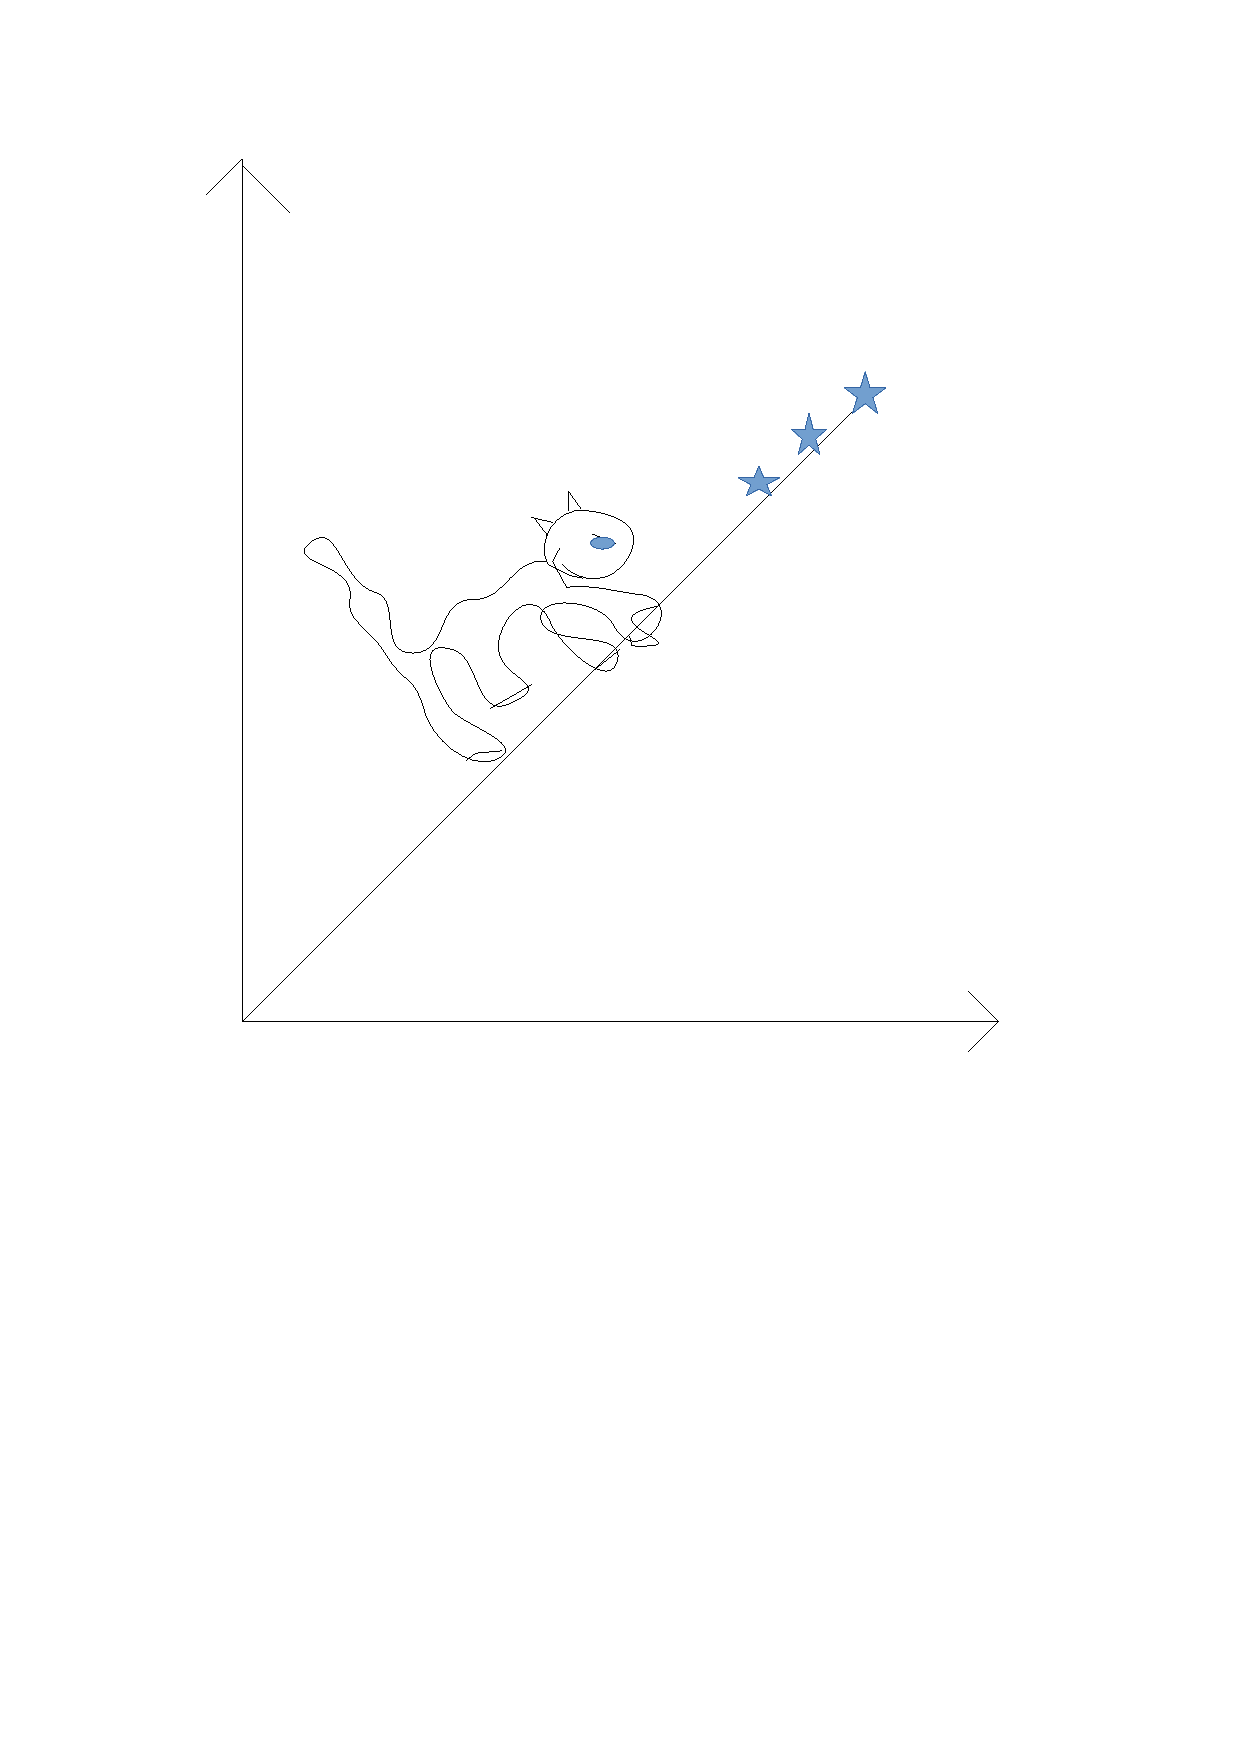
\includegraphics[width=0.45\textwidth]{kotek.pdf}
	\caption{Matematyczny kotek}
	\label{fig:kotek}
\end{figure}


\newpage
\addcontentsline{toc}{section}{Bibliografia}
\begin{thebibliography}{99}
\bibitem{topp} J.~Topp:
\emph{Algebra liniowa},
Wydawnictwo Uniwesytetu Gdańskiego, Gdańsk 2013
\\
\url{http://unixlab.iis.pwsz.elblag.pl/~j.topp/wp-content/uploads/2013/03/algebraliniowaUG.jpg}
\end{thebibliography}
                    \end{document}